\documentclass[a4paper, 11pt]{article}
\usepackage[english]{babel}
\usepackage[top=2cm,bottom=2cm,left=2cm,right=2cm]{geometry}
\usepackage[utf8]{inputenc}
\usepackage{import}
\usepackage{float}
\usepackage{subfigure}
% \usepackage{subfig}
\usepackage[pdftex]{graphicx}
% \usepackage{graphicx}
\usepackage{amssymb,amsmath,amsthm,amsfonts}
\usepackage{xspace}
\usepackage{tabularx}
\usepackage{indentfirst}
\usepackage{wrapfig,booktabs}
%\usepackage[small]{caption}
% \usepackage{subcaption}
\usepackage{eucal}
\usepackage{eso-pic}
\usepackage{hyperref}
\usepackage{url}
\usepackage{booktabs}
\usepackage{afterpage}
\usepackage{parskip}
\usepackage{listings}
\usepackage{fancyhdr}
\usepackage{textcomp}
\usepackage{cite}
\usepackage{multirow,multicol}
\usepackage{setspace}
\usepackage[version=4]{mhchem}
\usepackage{nicefrac}
\usepackage{siunitx}

\usepackage{caption}
\captionsetup{tableposition=top,font=small,width=0.8\textwidth}
%\usepackage[table]{xcolor}
\usepackage[arrowdel]{physics}
\usepackage{mathtools}
\usepackage{tablefootnote}
\usepackage{enumitem}

\setlist[description]{font={\scshape}} %style=unboxed,style=nextline
\usepackage{floatflt}
\usepackage{commath}
\usepackage{bm}
\usepackage{ifthen}
\usepackage{comment}
\usepackage[colorinlistoftodos,textsize=tiny]{todonotes}

\newcommand{\overbar}[1]{\mkern 1.5mu\overline{\mkern-1.5mu#1\mkern-1.5mu}\mkern 1.5mu}
\let\oldfrac\frac
\renewcommand{\frac}[3][d]{\ifthenelse{\equal{#1}{d}}{\oldfrac{#2}{#3}}{\nicefrac{#2}{#3}}}


\begin{document}

\title{Quantum Optics Lab report}
\author{Alessandro Lovo}

\maketitle

\begin{abstract}
  In this report, using the same experimental apparatus, three experiments regarding the quantum entanglement of photons will be performed: Entangled Quantum Key Distribution, Bell Inequality Violation and Quantum Tomography.
\end{abstract}


\section{Experimental apparatus}
  \begin{figure}[H]
    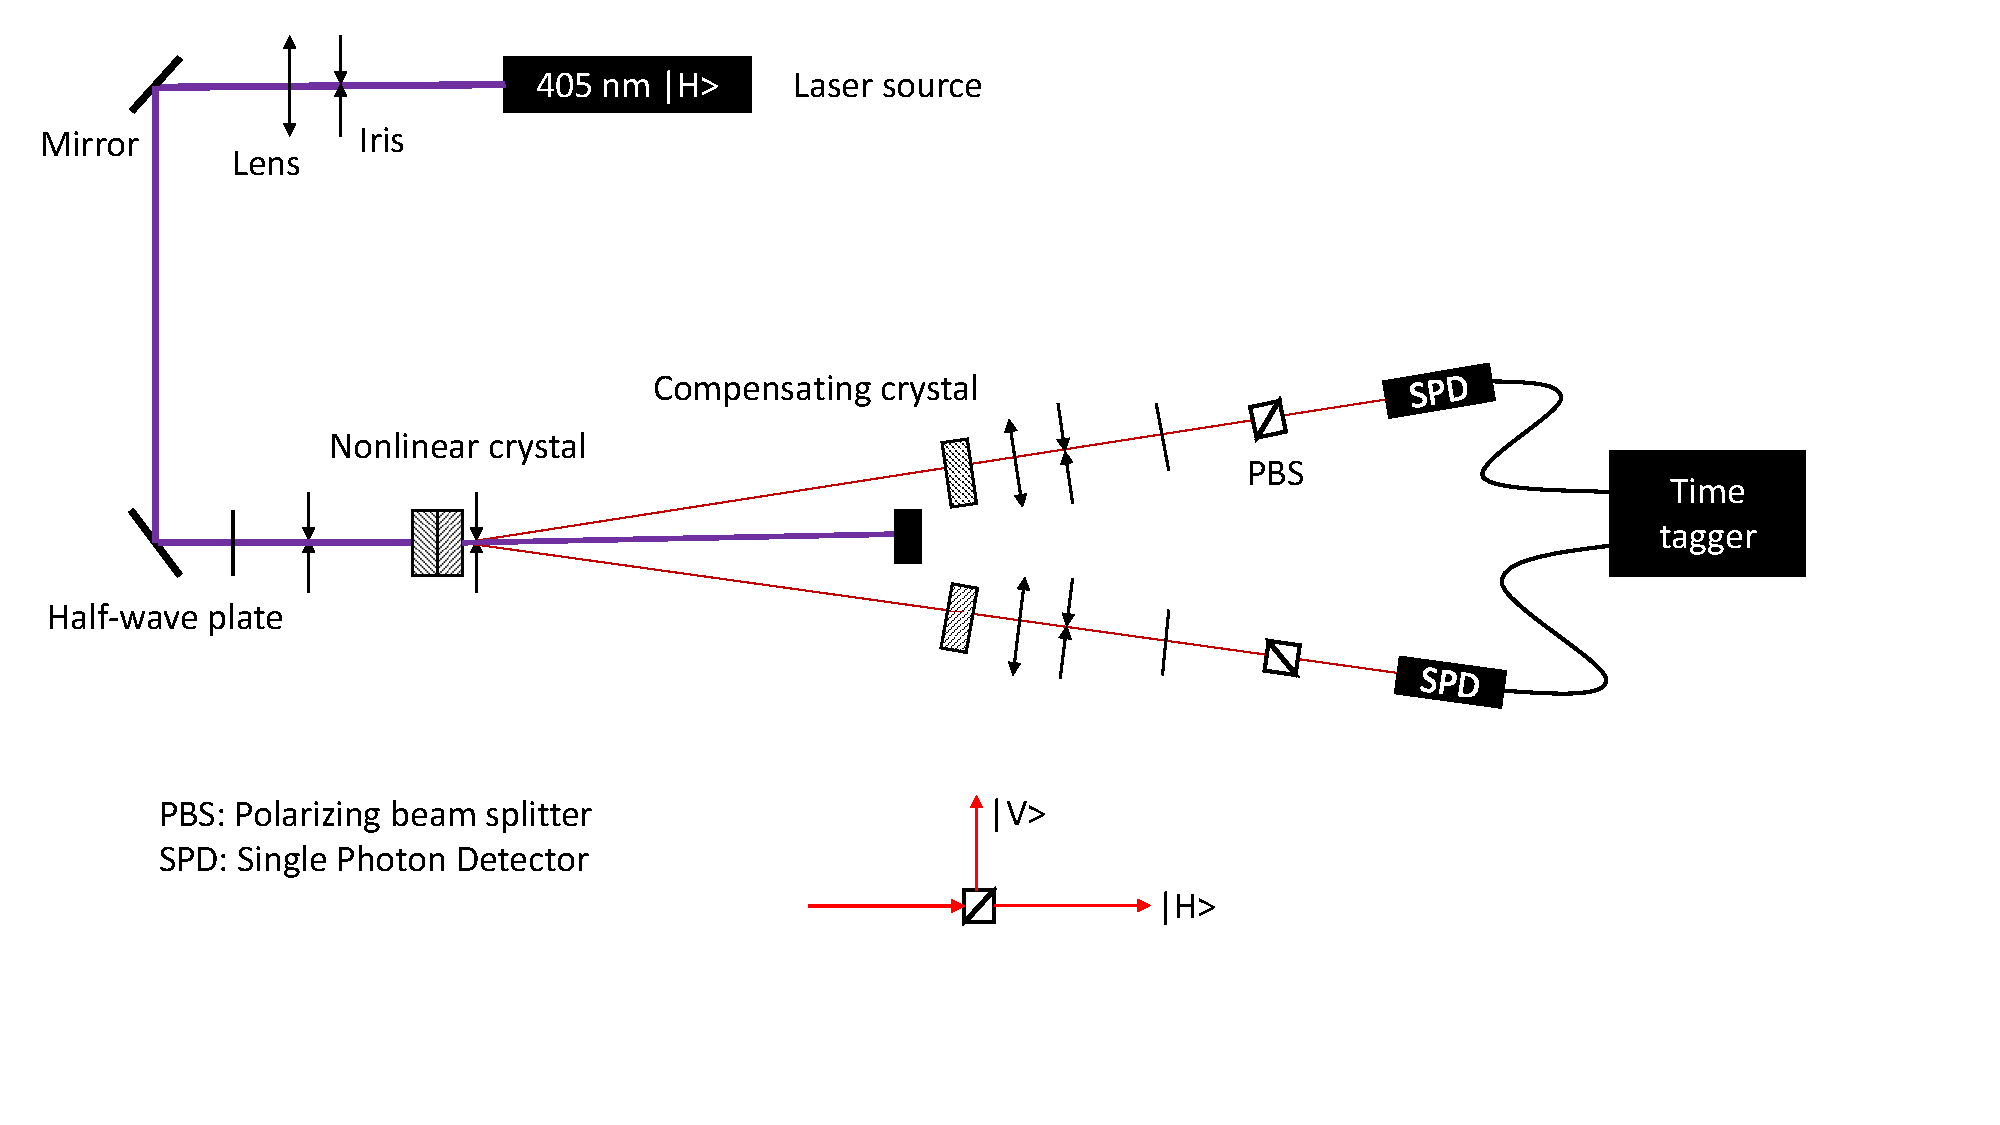
\includegraphics[width=1.0\textwidth]{img/apparatus.pdf}
    \caption{Schematics of the experimental apparatus.}
    \label{fig:apparatus}
  \end{figure}
  The schematics of the experimental apparatus are reported in fig \ref{fig:apparatus}: the source is a 405 \si{\nano\meter} laser whose beam is focused onto a nonlinear type II crystal obtained by sticking together two type I crystals with perpendicular optical axes. The laser emits light horizontally polarized ($\ket{H}$) and the two nonlinear crystals have a small chance ($\sim 10^{-7}$) of converting a photon in a pair of photons in the following way:
  \begin{gather*}
    \ket{H} \xrightarrow[]{\text{crystal 1}} \ket{VV} \quad
    \ket{V} \xrightarrow[]{\text{crystal 2}} \ket{HH}
  \end{gather*}
  Using the first half-wave plate the polarization of the beam is rotated to the diagonal state $\ket{D} = \frac{\ket{H} + \ket{V}}{\sqrt{2}}$, so when it impinges on the two crystals the exiting pair is in the entangled state $\ket{\phi^+} = \frac{\ket{HH} + \ket{VV}}{\sqrt{2}}$. However since the conversion is due to two type I crystals in order to not be able to distinguish which one did the conversion, two compensating crystals are introduced on the optical path. After some focusing the two beams hit the measuring device: a half-wave plate, a polarizing beam splitter (PBS) and a single photon detector (SPD).
  By tuning the angle $\alpha$ of the half-wave plate it is possible to measure any linear polarization $\ket{\theta} = \cos{\theta}\ket{H} + \sin{\theta}\ket{V}$ with the simple relation $\theta = 2\alpha$.
  The signals of the SPDs are sent to a time tagger in order to be able to do an a-posteriori coincidence analysis.

  \par{Coincidence analysis}
  The raw data of an acquisition consist of a list of timetags corresponding to the clicks of each of the two detectors expressed in timesteps of the time tagger $\tau = 80.955\si{.\pico\second}$. To extract the coincidences from it, first a histogram of the time differences between the two detectors is plotted and fitted with a gaussian with centroid $\mu$ and dispersion $\sigma$ (fig \ref{fig:hist}). At this point one can set a threshold $thr_{c} = 2\sigma$ for accepting coincidences, namely the number of coincidences $N$ is simply the number of points in the histogram for which $|\frac[f]{\Delta t}{\tau} - \mu| < thr_{c}$. To this value can then be assosciated a poissonian error $\sigma(N) = \sqrt{N}$.

  \begin{figure}[H]
    \centering
    \resizebox{0.7\textwidth}{!}{\import{img/}{coinc_hist_AA.pgf}}
    \caption{Example of histogram of the time differences between the two detectors; here both photons are measured in the state $\ket{A} = \ket{\frac[f]{-\pi}{4}}$. The red lines are drawn at $thr_c$.}
    \label{fig:hist}
  \end{figure}







\end{document}
